%%%%%%%%%%%%%%%%%%%%%%%%%%%%%%%%%%%%%%%%%
% Beamer Presentation
% LaTeX Template
% Version 1.0 (10/11/12)
%
% This template has been downloaded from:
% http://www.LaTeXTemplates.com
%
% License:
% CC BY-NC-SA 3.0 (http://creativecommons.org/licenses/by-nc-sa/3.0/)
%
%%%%%%%%%%%%%%%%%%%%%%%%%%%%%%%%%%%%%%%%%

%----------------------------------------------------------------------------------------
%	PACKAGES AND THEMES
%----------------------------------------------------------------------------------------

\documentclass{beamer}
\usepackage{subfigure}
\usepackage{amsmath}
\usepackage{mathtools}
\usepackage{listings}
\usepackage{multicol}
\usepackage{media9}

\makeatletter \@addtoreset{subfigure}{framenumber} \makeatother

\mode<presentation> {

% The Beamer class comes with a number of default slide themes
% which change the colors and layouts of slides. Below this is a list
% of all the themes, uncomment each in turn to see what they look like.

%\usetheme{default}
%\usetheme{AnnArbor}
%\usetheme{Antibes}
%\usetheme{Bergen}
%\usetheme{Berkeley}
%\usetheme{Berlin}
%\usetheme{Boadilla}
%\usetheme{CambridgeUS}
%\usetheme{Copenhagen}
%\usetheme{Darmstadt}
%\usetheme{Dresden}
%\usetheme{Frankfurt}
%\usetheme{Goettingen}
%\usetheme{Hannover}
%\usetheme{Ilmenau}
%\usetheme{JuanLesPins}
%\usetheme{Luebeck}
\usetheme{Madrid}
%\usetheme{Malmoe}
%\usetheme{Marburg}
%\usetheme{Montpellier}
%\usetheme{PaloAlto}
%\usetheme{Pittsburgh}
%\usetheme{Rochester}
%\usetheme{Singapore}
%\usetheme{Szeged}
%\usetheme{Warsaw}

% As well as themes, the Beamer class has a number of color themes
% for any slide theme. Uncomment each of these in turn to see how it
% changes the colors of your current slide theme.

%\usecolortheme{albatross}
%\usecolortheme{beaver}
%\usecolortheme{beetle}
%\usecolortheme{crane}
%\usecolortheme{dolphin}
%\usecolortheme{dove}
%\usecolortheme{fly}
%\usecolortheme{lily}
%\usecolortheme{orchid}
%\usecolortheme{rose}
%\usecolortheme{seagull}
%\usecolortheme{seahorse}
%\usecolortheme{whale}
%\usecolortheme{wolverine}

\setbeamertemplate{footline} % To remove the footer line in all slides uncomment this line
%\setbeamertemplate{footline}[page number] % To replace the footer line in all slides with a simple slide count uncomment this line

\setbeamertemplate{navigation symbols}{} % To remove the navigation symbols from the bottom of all slides uncomment this line
}

\usepackage{graphicx} % Allows including images
\usepackage{booktabs} % Allows the use of \toprule, \midrule and \bottomrule in tables

%----------------------------------------------------------------------------------------
%	TITLE PAGE
%----------------------------------------------------------------------------------------

\title[Short title]{Full Title of the Talk} % The short title appears at the bottom of every slide, the full title is only on the title page

\author{Kelsey Maass and Brisa Davis} % Your name
\institute[UW] % Your institution as it will appear on the bottom of every slide, may be shorthand to save space
{
AMATH 574 \\ % Your institution for the title page \\
Group 6
\medskip
}
\date{\today} % Date, can be changed to a custom date

\begin{document}

\begin{frame}
\titlepage % Print the title page as the first slide
\end{frame}

\begin{frame}
\frametitle{Introduction} 
Kelsey
\end{frame}

%----------------------------------------------------------------------------------------
%	PRESENTATION SLIDES
%----------------------------------------------------------------------------------------

\begin{frame}
\frametitle{LWR}
Kelsey
\end{frame}

%------------------------------------------------

\begin{frame}
\frametitle{PW}
Intro, Kelsey. Eigenvectors and values
\end{frame}

%------------------------------------------------

%------------------------------------------------

\begin{frame}
\frametitle{PW: Hugoniot Loci}
From this system, the Rankine-Hugoniot condition 
\begin{align*}
s(q_* - q ) = f(q_*)-f(q)
\end{align*}
gives us the two equations 
\begin{align*}
&s(\rho_* - \rho ) = \rho_*v_* - \rho v, \\
&s (\rho_*v_* - \rho v ) = \rho_*v_*^2 + p(\rho) - \rho v^2 - p(\rho).
\end{align*}
From these two equations
the equation for the Hugoniot loci can be found to be
\begin{align*}
\rho v = \rho v_* \pm \rho \sqrt{\left( \rho - \rho_*\right) \left( p(\rho ) - p(\rho_*)\right) / \rho_*\rho }.
\end{align*}

\end{frame}

\begin{frame}
\frametitle{PW: Hugoniot Loci}
Plotting this equation 
\begin{align*}
\rho v = \rho v_* \pm \rho \sqrt{\left( \rho - \rho_*\right) \left( p(\rho ) - p(\rho_*)\right) / \rho_*\rho }.
\end{align*}
gives
\begin{figure}[h!]
 \centering
  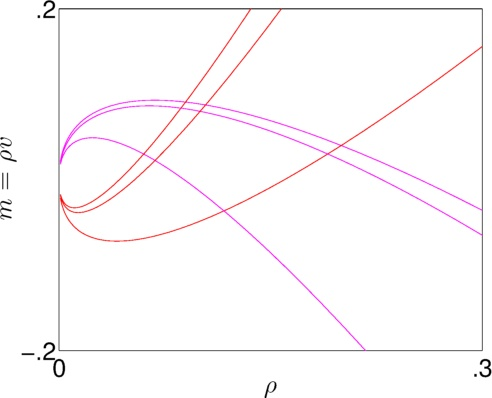
\includegraphics[width=45mm]{../MatlabCode/Images/PW_Loci.jpg}
\end{figure}
Here, $\lambda_1$ loci are shown in magenta and $\lambda_2$ loci are shown in red.
\end{frame}

\begin{frame}
\frametitle{PW: Integral Curves}
Using $p(\rho) = \rho^{\gamma}$ for $\gamma \neq 1$, since this is the value used in the AR model we will examine later, the equations for the integral curves can be found to be
\begin{align*}
\rho v = \rho v_* + \frac{2 \rho}{\gamma - 1}\left( \sqrt{p'(\rho_*)} - \sqrt{p'(\rho)}\right)
\end{align*}
for $\lambda_1$, and 
\begin{align*}
\rho v = \rho v_* + \frac{2 \rho}{\gamma - 1}\left( \sqrt{p'(\rho)} - \sqrt{p'(\rho_*)} \right)
\end{align*}
for $\lambda_2$.
\end{frame}

\begin{frame}
\frametitle{PW: Integral Curves}
Plotting these curves gives
\begin{figure}[h!]
 \centering
  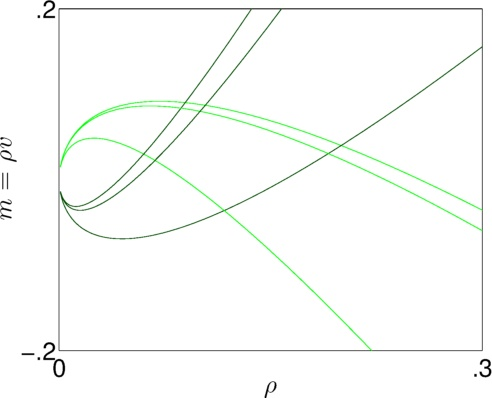
\includegraphics[width=45mm]{../MatlabCode/Images/PW_IntegralCurves.jpg}
\end{figure}
Here, $\lambda_1$ integral curves are shown in light green and $\lambda_2$ integral curves are shown in dark green.
\end{frame}

\begin{frame}
\frametitle{PW: Areas of Validity}
Restrictions on the way that $\lambda$ must vary across a wave allow us to identify the regions of the Hugoniot loci and integral curves that are valid for any given point. \\
\vspace{0.1in}
Shocks:
\begin{align*}
q_l \rightarrow q_r \hspace{0.2in}&: \hspace{0.2in} \lambda \textnormal{ must decrease}\\
q_r \rightarrow q_l \hspace{0.2in}&: \hspace{0.2in} \lambda \textnormal{ must increase}
\end{align*}
Rarefaction:
\begin{align*}
q_l \rightarrow q_r \hspace{0.2in}&: \hspace{0.2in} \lambda \textnormal{ must increase}\\
q_r \rightarrow q_l \hspace{0.2in}&: \hspace{0.2in} \lambda \textnormal{ must decrease}
\end{align*}
\end{frame}

\begin{frame}
\frametitle{PW: Areas of Validity}
Using this, we can determine the valid curves:
\begin{figure}[h!]
 \centering
 \subfigure[Valid curves for a point $q_l$.]{
  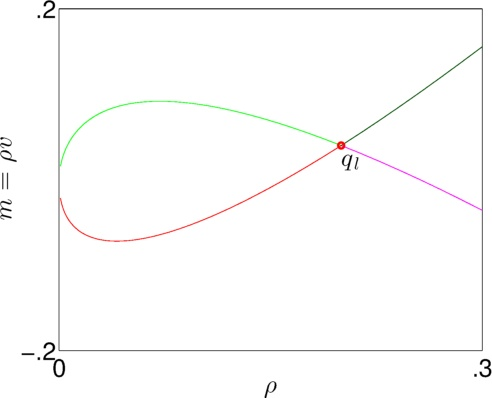
\includegraphics[width=45mm]{../MatlabCode/Images/PW_validStateCurvesLeft.jpg}
   }
 \subfigure[Valid curves for a point $q_r$.]{
  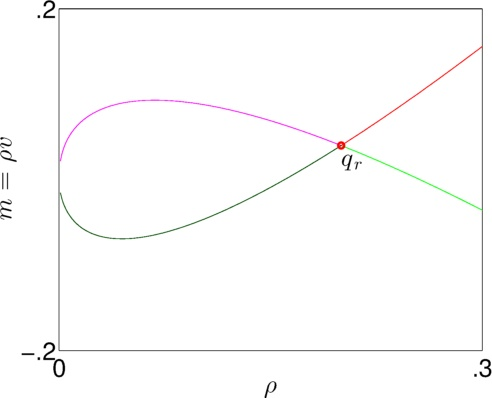
\includegraphics[width=45mm]{../MatlabCode/Images/PW_validStateCurvesRight.jpg}
   }
  \label{fig:PW_curves}
\end{figure}

Here, shocks are shown in red or magenta and rarefaction waves are shown in either light or dark green.

\end{frame}

%------------------------------------------------

%------------------------------------------------

\begin{frame}
\frametitle{AR}
Intro, Kelsey. Eigenvectors and values
\end{frame}

%------------------------------------------------

%------------------------------------------------

\begin{frame}
\frametitle{AR: Hugoniot Loci}
In order to consider the Hugoniot loci for this system we must first write the system in conservation form. 
With some manipulation, we can get the system
\begin{align*}
&\partial_t\rho + \partial_x(\rho v) = 0, \\
&\partial_t \left(\rho\left(v + p(\rho )\right)\right) + \partial_x \left( \rho v\left(v + p(\rho )\right)\right) = 0.
\end{align*}
This can be rewritten as $q_t + f(q)_x = $ by defining
\begin{align*}
q = \left[ \begin{matrix}
\rho \\ y
\end{matrix}\right], \hspace{0.3in}
f(q) = \left[ \begin{matrix}
v\rho \\
vy
\end{matrix}\right].
\end{align*}
where $y = \rho\left(v + p(\rho )\right)$.
\end{frame}

\begin{frame}
\frametitle{AR: Hugoniot Loci}
From the Rankine-Hugoniot condition
\begin{align*}
s(q_*- q) = f(q_*) - f(q).
\end{align*}
we get the two equations
\begin{align*}
s(\rho_* - \rho) = v_*\rho_* - v\rho,\\
s(y_* - y) = v_*y_* - vy.
\end{align*}
From these equations, the equations for the Hugoniot loci can be found to be
\begin{align*}
&\rho v = \rho \left( v_* + p(\rho_*)\right) - \rho p(\rho)),\\
&\rho v = \rho_* v_*,
\end{align*}
corresponding to $\lambda_1$ and $\lambda_2$, respectively.
\end{frame}

\begin{frame}
\frametitle{AR: Integral Curves}
In order to consider the integral curves for this system \cite{AwRascle2000} 
works from the system
\begin{align*}
&\partial_t \rho + \partial_x (\rho v) = 0, \\ 
&\partial_t v + \left(v - p'(\rho)\rho\right)\partial_x v = 0.
\end{align*}
After working with these equations to find the integral curves, you find that they coincide with the Hugoniot loci.
\end{frame}

\begin{frame}
\frametitle{AR: Curves}
Plotting these curves gives:
\begin{figure}[h!]
    \subfigure[$\lambda_1$-curves in the M plane.]{
  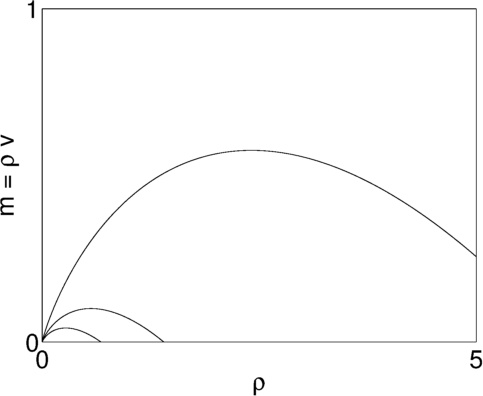
\includegraphics[width=45mm]{../MatlabCode/Images/HLIC_M_lamb1.jpg}
   }
 \subfigure[$\lambda_2$-curves in the M plane.]{
  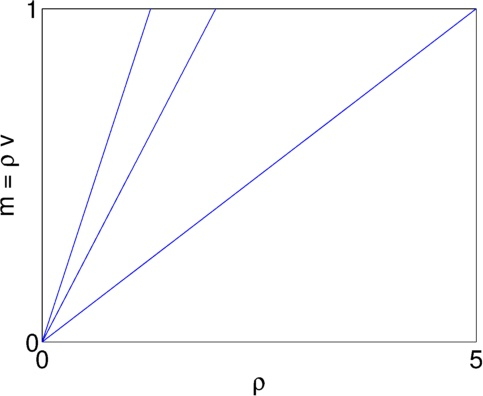
\includegraphics[width=45mm]{../MatlabCode/Images/HLIC_M_lamb2.jpg}
   }
     \label{fig:AR_curves}
\end{figure}

\end{frame}

\begin{frame}
\frametitle{AR: Areas of Validity}
Restrictions on the way that $\lambda$ must vary across a wave allow us to identify the regions of the Hugoniot loci and integral curves that are valid for any given point. \\
\vspace{0.1in}
Shocks:
\begin{align*}
q_l \rightarrow q_r \hspace{0.2in}&: \hspace{0.2in} \lambda \textnormal{ must decrease}\\
q_r \rightarrow q_l \hspace{0.2in}&: \hspace{0.2in} \lambda \textnormal{ must increase}
\end{align*}
Rarefaction:
\begin{align*}
q_l \rightarrow q_r \hspace{0.2in}&: \hspace{0.2in} \lambda \textnormal{ must increase}\\
q_r \rightarrow q_l \hspace{0.2in}&: \hspace{0.2in} \lambda \textnormal{ must decrease}
\end{align*}
\end{frame}

\begin{frame}
\frametitle{AR: Areas of Validity}
Using this, we can determine the valid curves:
\begin{figure}[h!]
 \subfigure[Valid waves for the point $q_l$.]{
  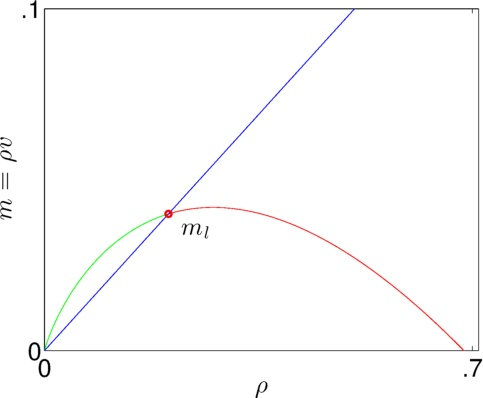
\includegraphics[width=45mm]{../MatlabCode/Images/Validity_M_ql.jpg}
   }
 \subfigure[Valid waves for the point $q_r$.]{
  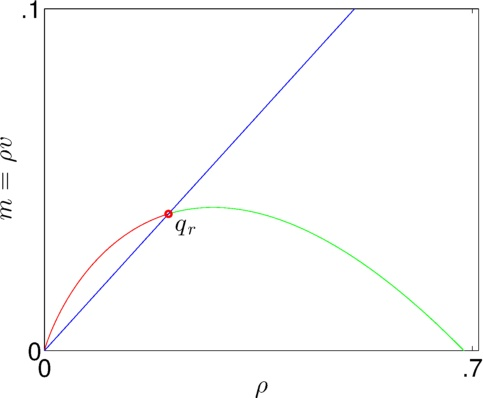
\includegraphics[width=45mm]{../MatlabCode/Images/Validity_M_qr.jpg}
   }
\end{figure}
Here, shocks are shown in red, rarefaction waves are shown in green, and the contact discontinuity is shown in blue.
\end{frame}

%------------------------------------------------

%------------------------------------------------

\begin{frame}
\frametitle{Examples}

To illustrate a couple of examples where the AR model preforms better than the PW model, consider two different examples: 
\begin{table}[t]
\caption{Initial values used in examples 1 and 2.}
\begin{center}
\begin{tabular}{| c | c c  c c|}
\hline
& $v_l$ & $\rho_l $ & $v_r$ & $\rho_r $\\
\hline
Example 1 & 0.2 & .03 & 0.3 & 0.4 \\
Example 2 & 0 & 0 & 0.3 & 0.4\\
\hline
\end{tabular}
\end{center}
\end{table}
\end{frame}

\begin{frame}
\frametitle{Example 1}
The solution to the Riemann problem is:
\begin{figure}[h!]
 \centering
 \subfigure[Solution from the AR model.]{
  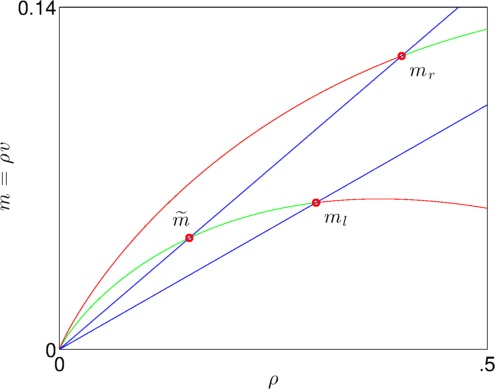
\includegraphics[width=45mm]{../MatlabCode/Images/AR_example1.jpg}
   }
    \subfigure[Solution from the PW model.]{
  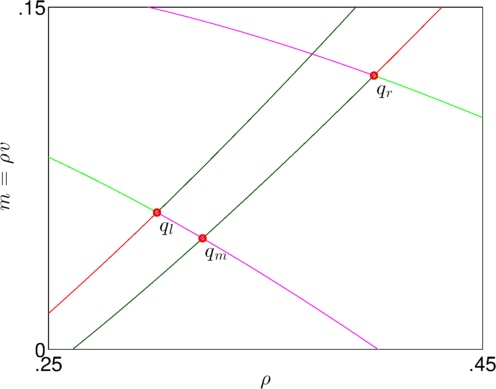
\includegraphics[width=45mm]{../MatlabCode/Images/PW_example1.jpg}
   }
\end{figure}
\end{frame}

\begin{frame}
\frametitle{Example 1}
\begin{center}
\begin{multicols}{2}%
AR model:
\includemedia[
  width=0.9\linewidth,
  height=0.7\linewidth,
  activate=pageopen,
  addresource=AR_Example1Movie.mp4,
  flashvars={source=AR_Example1Movie.mp4}
]{}{VPlayer.swf}
\vfill
\columnbreak
PW Model:
\includemedia[
  width=0.9\linewidth,
  height=0.7\linewidth,
  activate=pageopen,
  addresource=PW_Example1Movie.mp4,
  flashvars={source=PW_Example1Movie.mp4}
]{}{VPlayer.swf}
\end{multicols}
\end{center}
\end{frame}

\begin{frame}
\frametitle{Example 2}
The solution to the Riemann problem is:

\begin{figure}[h!]
 \centering
 \subfigure[Solution from the AR model.]{
  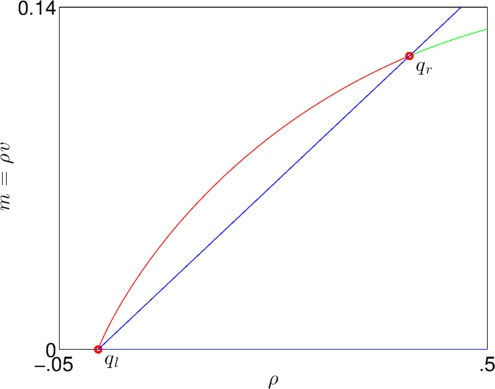
\includegraphics[width=45mm]{../MatlabCode/Images/AR_example2.jpg}
   }
 \subfigure[Solution from the PW model.]{
  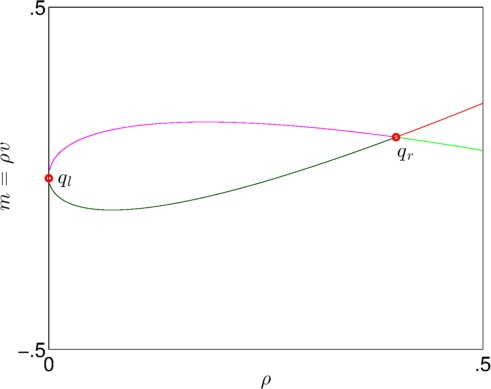
\includegraphics[width=45mm]{../MatlabCode/Images/PW_example2.jpg}
   }
\end{figure}
\end{frame}

\begin{frame}
\frametitle{Example 2}
\begin{center}
\begin{multicols}{2}%
AR model:
\includemedia[
  width=0.9\linewidth,
  height=0.7\linewidth,
  activate=pageopen,
  addresource=AR_Example2Movie.mp4,
  flashvars={source=AR_Example2Movie.mp4}
]{}{VPlayer.swf}
\vfill
\columnbreak
PW Model:
\includemedia[
  width=0.9\linewidth,
  height=0.7\linewidth,
  activate=pageopen,
  addresource=PW_Example2Movie.mp4,
  flashvars={source=PW_Example2Movie.mp4}
]{}{VPlayer.swf}
\end{multicols}
\end{center}
\end{frame}

%------------------------------------------------

\begin{frame}
\Huge{\centerline{Questions?}}
\end{frame}

%----------------------------------------------------------------------------------------
\bibliography{presentation}{}
\bibliographystyle{plain}
\end{document} 